%%%%%%%%%%%%%%%%%%%%%%%%%%%%%%%%%%%%%%%%%%%%%%%%%%%%%
\documentclass[apj]{emulateapj}
%\documentclass[preprint2]{aastex61}
%\documentclass[12pt,preprint]{aastex}
\graphicspath{{figures/}}
\DeclareGraphicsExtensions{.jpg,.pdf,.png,.eps,.ps}

\usepackage[table,usenames,dvipsnames]{xcolor}
\usepackage{amsmath}
\usepackage{subfigure}
\usepackage[backref,breaklinks,colorlinks,citecolor=blue]{hyperref}
\usepackage{natbib}
%\usepackage{natbib}
\bibliographystyle{fapj}
\usepackage{graphicx}
\usepackage{multirow}
\usepackage{soul}

%\newcommand{\jcap}{JCAP}

\newcommand{\sqdeg}{deg$^2$ }
\newcommand{\omb}{\ensuremath{\Omega_b h^2}}
\newcommand{\omc}{\ensuremath{\Omega_c h^2}}
\newcommand{\clpp}{\ensuremath{C_{L}^{\phi\phi}}}
\newcommand{\cpmf}{\ensuremath{C_{\ell}^{\rm PMF}}}

\newcommand{\cpmftens}{\ensuremath{C_{\ell}^{\rm PMF,\,tens}}}
\newcommand{\cpmfvec}{\ensuremath{C_{\ell}^{\rm PMF,\,vec}}}
\newcommand{\apmf}{\ensuremath{A_{\rm PMF}}}
\newcommand{\bpmf}{\ensuremath{B_{\rm 1\,Mpc}}}
\newcommand{\alens}{\ensuremath{A_{\rm lens}}}
\newcommand{\lcdm}{\ensuremath{\Lambda}CDM}
\newcommand{\nrun}{\ensuremath{n_{\rm run}}}
\newcommand{\neff}{\ensuremath{N_{\rm eff}}}
\newcommand{\ho}{H\ensuremath{_0}}
\newcommand{\mnu}{\ensuremath{\sum m_\nu}}
\newcommand{\ukarcmin}{\ensuremath{\mu}{\rm K-arcmin}}
\newcommand{\lknee}{\ensuremath{\ell_{\rm knee}}}
\newcommand{\lcut}{\ensuremath{\ell_{\rm cut}}}
\newcommand{\fermilat}{\textit{Fermi}-LAT}

\newcommand{\be}{\begin{equation}}
\newcommand{\ee}{\end{equation}}
\newcommand{\planck}{{\sl Planck}}
\newcommand{\wmap}{{\sl WMAP}}
\newcommand{\bicepkeck}{BICEP2/Keck Array}
\newcommand{\sptnew}{SPT-3G}
\newcommand{\pb}{\textsc{Polarbear}}
\newcommand{\simons}{Simons Array}
\newcommand{\sptpol}{SPTpol}
\newcommand{\advactpol}{Adv.~ACTpol}

\newcommand{\tbd}[1]{\textcolor{Red}{{\bf TBD}: #1}}
\newcommand{\gab}[1]{\textcolor{Orchid}{[{\bf GS}: #1]}}
\newcommand{\changed}[1]{\textcolor{Red}{#1}}
\newcommand{\removed}[1]{\textcolor{Red}{}}
\include{number_list}

%

% ref to section \S\ref{sec:label}

%\submitjournal{ApJ}
\def\Melbourne{1}
\def\uci{2}
%%%%%%%%%%%%%%%%%%%%%%%%%%%%%%%%%%%%%%%%%%%%%%%%%%%%%
\begin{document}

\title{Cosmic Microwave Background Power Spectra from Few Bit Timestreams}
\author{L.~Balkenhol\altaffilmark{\Melbourne} and C.~L.~Reichardt\altaffilmark{\Melbourne}}
\altaffiltext{\Melbourne}{School of Physics, University of Melbourne, Parkville, VIC 3010, Australia}
\email{christian.reichardt@unimelb.edu.au}

\begin{abstract}

Observations of the Cosmic Microwave Background (CMB) are of significant value to modern cosmology and particle physics. The large size of time-ordered-data (TOD) being recorded causes new challenges in hardware design, mission planning and analysis for future CMB experiments. These issues are particularly significant for Antarctica- and space-based experiments which depend on satellite links to transmit their data. We explore the viability of reducing the TOD to few-bit numbers to address these issues. Unlike lossless compression, this technique introduces additional noise into the data. We present a set of one, two, and three bit digitisation schemes and determine the degradation the compression causes in temperature and polarisation power spectra. The added noise has no dependence on the multipole moment $\ell$ for white and $1/f$ detector noise. The compression performs equally for temperature and polarisation observations and scales the same way as detector noise with depth of observation. Three bit digitisation has a percent-level contribution to the map noise level. Such digitisation is a promising strategy for upcoming experiments.

\end{abstract}

%C: maybe sub techniques:misc for methods: data analysis ? unfortunately no data compression tag
\keywords{cosmic background radiation --- polarization --- techniques: miscellaneous}
\section{Introduction}
\label{sec:intro}

Observations of the Cosmic Microwave Background (CMB) have played a key role in physics since its discovery \citep{penzias1965}. Current and future study of the information it contains will put tight constraints on cosmological models. Upcoming science goals include the discovery of inflationary gravitational waves, construction of precise lensing maps and thorough studies of the Sunyaev-Zeldovich (SZ) effects. Additionally, the CMB probes structure formation, reionisation and is a powerful test for dark matter and dark energy models. Lastly, the relativistic number of species and the neutrino mass sum are measured by CMB experiments \citep{s4sciencebook, core2011, litebird2016, pixie2011}. 

The CMB community has developed a variety of compression techniques and computational approaches to handle the increasing volume of data \citep{tristam2007}. These include the compression of time-ordered data (TOD) into maps \citep{tegmark1997}, bandpower estimation \citep{tegmark1998} and the pseudo $C_l$ method \citep{brown2005}.

A potential hurdle for experiments at remote locations are the transmission limitations of satellite links. Space-based experiments have employed a combination of lossless and lossy compression techniques, including reduced bits in the TOD \citep{gaztanaga1998, maris2003}. Antarctica-based experiments that transmit a portion of their data via a satellite link have downsampled their data in the past to meet telemetry allocations and have not yet used few bit digitisation of the TOD. As we approach the next generation of ground-based experiments, CMB-S4, and the launch of new space-based missions (LiteBIRD, PIXIE, COrE+), we must consider potential transmission bottlenecks carefully. %C: Is there a reference detailing downsampling of SPT data?

In this work we present the method of extreme digitisation, which reduces a many bit (often 32 or 64 bit) signal to a few bits for ground-based experiments. We apply extreme digitisation to the TOD and detail the resulting effects on temperature and polarisation power spectra. We find that an optimal three bit digitisation scheme adds $<1.7\%$ to the map noise level.

This work is structured as follows. In \S\ref{sec:dig} we detail the challenges that come with handling large data volumes, introduce the process of extreme digitisation and lay out the framework used to test its performance. We describe the power spectrum estimation and present the results in section \S\ref{sec:results}. We summarise our findings in \S\ref{sec:conclusions}.

%This work is structured as follows. We detail the arising challenges in handling large TOD in \S\ref{subsec:problem}. We subsequently formulate extreme digitisation in \S\ref{subsec:extremedigitisation} and lay out the framework used to test its performance in \S\ref{subsec:method}. The details of the power spectrum estimation used are laid out in \S\ref{subsec:psestimation}. We continue by presenting the noise induced through the dicitisation process in \S\ref{subsec:additionalnoise} and summarise our findings in \S\ref{sec:conclusions}. 

%CMB is great; One reason is that there is a history of compression and computational techniques that reduce the load of large datasets. ie maps; bandpowers; pseudo-cls.

%satellites have also reduced bits on TOD; ground based haven't had to yet

%however as we discuss building ever larger arrays at remote sites, we are starting to be limited: spt example.

%in this work we present digitisation for ground-based cmb polarisation measurements.
%teaser results


%The outline of this paper is as follows. 
%We present the digisation schemes in \S\ref{sec:dig}, and their performance in \S\ref{sec:results}
%We summarize our findings in \S\ref{sec:conclusions}. 

\section{Digitisation}
\label{sec:dig}

\subsection{The Challenges Of Large Data Sets}
\label{subsec:problem}

%Data influx + Transmission

The science goals of upcoming CMB experiments depend on achieving substantially faster mapping speeds. This has lead to the number of detectors of ground-based experiments following a Moore's law like trend, doubling approximately every 2 years \citep{s4sciencebook, Abazajian2015}. The growing detector count translates into an exponential growth in data volume.

Excellent conditions for CMB observations can be found in space and at various locations on earth, including the South Pole \citep{kovac2007}. Space- and Antarctica-based experiments depend on satellite transmission. The South Pole will continue its contribution to CMB science in the next generation of ground-based instruments, which aims to collect 2 million detector years in total. During CMB-S4 observations at the South Pole site will face a data influx of $\sim \mathcal{O}(10)\mathrm{Tb/d}$. However, the current transmission allocation for SPT-3G is $150\mathrm{Gb/d}$, which will likely see only a moderate increase. The transmission bottleneck is currently overcome by recovering the full data on hard drives with some latency and transmitting a downsampled version of the data. The downsampling process loses high frequency information and continued usage of it will narrow the information window decisively, prohibiting high multipole moment science to be carried out on the transmitted data set. This also means that any potential faults or errors in the experiment apparent in this range are not visible in the transmitted data. %C: Is there a paper detailing trasmission limits for SPT and that the data is currently downsampled?

The Planck mission has demonstrated the merits of carrying out CMB observations from space \citep{planck2018}. Upcoming missions aim to exceed the detector count of Planck by at least an order of magnitude \citep{litebird2014, pixie2011, core2018}. Strategies to meet the telemetry specifications of each mission appear to be in development. It is not clear whether the data compression knowledge developed during the Planck mission will guarantee optimal performance for future satellites. Each mission will most likely have to carefully construct a compression algorithm through a combination of lossless and lossy techniques specific to their requirements.

%Planning

Beyond transmission challenges, mission planning is becoming exceedingly difficult. Full simulation of TOD over the entire parameter space of detection scenarios is the desired way to decide on CMB-S4 configurations. Given the shear size of TOD expected, this is not possible \citep{s4sciencebook}. Ground-based observations have to rely on different planning strategies or aim to reduce the size of the TOD in order to maximise the productivity of the design stage. Space-based missions carry out a similar analysis specific to their instruments to heighten their science output.

% Analysis

Operations on the TOD, such as noise-removal and map-making are a vital part of CMB data analysis. While we have not experienced the limitations of the accessible computational assets, the exponential growth of CMB data makes its analysis increasingly expensive.

%why is it worth considering

Extreme Digitisation would tackle the challenges mentioned above by reducing TOD volume by an order of magnitude. Together with already established lossless compression techniques (e.g. FLAC, run-length coding, Huffman coding, etc.) this addresses transmission hurdles. Beyond that extreme digitisation has the potential of easing issues in planning, analysis and hardware requirements.

%what others have done

While the advantages of using few bit TOD in space-based CMB observations have been demonstrated by the Planck mission \citep{maris2003}, other science areas have also shown the power of this tool. \cite{jenet1998} explored the application of such compression to radio pulsar timing measurements with success. Recently Clearwater et al. (private communication) have demonstrated the advantages of using one and two bit data when searching for continuous gravitational waves using the Laser Interferometer Gravitational-Wave Observatory (LIGO).


\subsection{Extreme Digitisation}
\label{subsec:extremedigitisation}

Digitisation is a lossy compression technique. However, the additional noise depends on the details of the digitisation scheme and the input signal. There is usually little concern around finding an optimal set of digitisation parameters as it is common to have access to large numbers of bits to store information, where changes in the digitisation scheme become insignificant to the distortion induced. It is in our interest however to consider extreme, i.e. few bit, digitisation. In this case the digitisation scheme must be carefully constructed. We review the key aspedcts of designing digitisation schemes as edtablished by \cite{max1960} below.

Digitisation discretises an input signal by sorting it into $N$ appropriate ranges, such that an input between $x_i$ and $x_{i+1}$ produces an output at $y_i$. The set of parameters $N, x_i, y_i$ fully specify a digitisation scheme. Conventionally one chooses $x_{1} = -\infty$ and $x_{N+1} = \infty$. In order to quantify the performance of a given digitisation scheme we define the distortion as

\begin{equation} D = \left\langle  \left( s - \hat{s} \right)^2 \right\rangle, \end{equation}

where $s$ is the input and $\hat{s}$ the output signal. For an input signal that has a stochastic element we introduce the input amplitude probability density $p(x)$. This allows us to rewrite the above as

\begin{equation} D = \sum_{i = 1}^N \int_{x_i}^{x_{i+1}} \left(x-y_i\right)^2 p(x) dx. \end{equation}

Since we wish to minimise the distortion we differentiate the distortion with respect to $x_i$ and $y_i$ and set the derivatives to zero. We obtain the two equations

\begin{equation} \label{eq:distderiv1}
\frac{\partial D}{\partial x_i} = \left(x_i-y_{i-1}\right)^2 p(x_i) - \left(x_i - y_i\right)^2 p(x_i) = 0,
\end{equation}

\begin{equation} \label{eq:distderiv2}
\frac{\partial D}{\partial x_j} = -2 \int_{x_i}^{x_{i+1}} \left( x-y_i \right) p(x) dx = 0.
\end{equation}

Rearranging equation \ref{eq:distderiv1} we deduce

\begin{equation} \label{eq:digitequalspacecondition}
x_i = \frac{y_i+y_{i+1}}{2},
\end{equation}

which informs us that an output level $y_i$ must lie halfway between its delimiting thresholds $x_i$ and $x_{i+1}$. From equation \ref{eq:distderiv2} we gain the additional condition

\begin{equation} \label{eq:digitareacondition}
\int_{x_i}^{x_{i+1}} \left( x-y_i \right) p(x) dx = 0.
\end{equation}

This implies that we should choose $y_i$, such that it halves the area underneath $p(x)$ in the interval from $x_i$ to $x_{i+1}$.

To progress further we have to make an assumption about the probability distribution of input signals. We take ground-based CMB observations to operate at low signal to noise and assume detector noise to be gaussian white. The input is then purely stochastic and  $p(x) = (1/\sqrt{2\pi\sigma^2}) e^{-x^2/2\sigma^2}$, where $\sigma$ is the standard deviation of the detector noise. Under these assumptions the system of equations can be solved numerically. One begins by picking $y_1$ and calculating the remaining $x_i$'s and $y_i$'s using equation \ref{eq:digitequalspacecondition}. Afterwards one checks whether this choice of values satisfy the conditions given by equation \ref{eq:digitareacondition}. If that is the case, the $x_i$'s and $y_i$'s were chosen appropriately.

We use the findings of \cite{max1960} to formulate the multi-level functions we use for one, two, and three bit digitisation. Given an input signal $s(t)$ a digitisation scheme using $N$ bits returns the output $\hat{s}_N(t)$. For one bit digitisation we apply the sign function

\begin{equation} \label{eq:1bit}
\hat{s}_1(t) = \left\{ \begin{array}{lr}
1, & \text{for } s(t) > 0\\
-1, & \text{for } s(t) \leq 0
\end{array} \right. \end{equation}

to the TOD. For two bit digitisation we apply the four-level function

\begin{equation}  \label{eq:2bit}
\hat{s}_2(t) = \left\{ \begin{array}{rl}
1.51 \sigma, & \text{for } s(t) \geq 0.9816 \sigma\\
0.4528 \sigma, & \text{for } 0 \leq s(t) < 0.9816 \sigma\\
-0.4528 \sigma, & \text{for } -0.9816 \sigma \leq s(t) < 0\\
-1.51 \sigma, & \text{for } -0.9816 \sigma < s(t)\\
\end{array} \right. . \end{equation}
%C: should i round to equal significant figures here? Unfortunately these are the exact values that i used...

Finally the optimal three bit digitisation is described by the eight-level function

\begin{equation}  \label{eq:3bit}
\hat{s}_3(t) = \left\{ \begin{array}{rl}
2.152 \sigma, & \text{for } s(t) \geq 1.748 \sigma\\
1.344 \sigma, & \text{for } 1.05 \sigma \leq s(t) < 1.748 \sigma\\
0.756 \sigma, & \text{for } 0.501 \sigma \leq s(t) < 1.05 \sigma\\
0.245 \sigma, & \text{for } 0 \leq s(t) < 0.501 \sigma\\
-0.245 \sigma, & \text{for } -0.501 \sigma \leq s(t) < 0\\
-0.756 \sigma, & \text{for } -1.05 \sigma \leq s(t) < -0.501 \sigma\\
-1.344 \sigma, & \text{for } -1.748 \sigma \leq s(t) < -1.05 \sigma\\
-2.152 \sigma, & \text{for } -1.748 \sigma < s(t)\\
\end{array} \right. . \end{equation}

The fact that the single bit digitisation scheme makes no references to the standard deviation of the signal is irrelevant. This affects the normalisation of the output, which we can account for during later analysis as demonstrated in the appendix. What is important is the spacing between digitisation thresholds and between output levels.

%Completely different digitisation schemes can be thought of, which would for example reference the most drastic outlier in the data set, or seek to place equal numbers of points into each digitisation level. However, given the assumptions made the schemes derived above minimise the distortion metric defined. Additionally, they are simple enough to be easily implemented computationally. We consider how to design digitisation schemes that preserve the power of the TOD and how to adjust a given digitisation scheme to ensure power conservation in the appendix.

\subsection{Methods}
\label{subsec:method}

To investigate the performance of the derived digitisation schemes we simulate many scans over CMB template maps at the timestream level. We obtain control maps that use 64 bit TOD and maps that have undergone one, two, and three bit digitisation of the TOD. We calculate the temperature and polarisation power spectra of each map and determine the noise level.
%C: Do I need to mention that we assume to have an infinitely fast spinning plate?

To create the template maps we use the Hierarchical Equal Area isoLatitude Pixelization of a sphere \citep[HEALPix;][]{healpix}\footnote{Available at \url{http://healpix.sourceforge.net/}} framework. We generate a realisation of I, Q and U maps with $\mathrm{NSIDE} = 4096$ based on the 2015 results of the Planck collaboration. The key cosmological parameters are $\Omega_b \approx 0.049 $, $\Omega_c \approx 0.265$, $\Omega_m \approx 0.316$ and $h \approx 0.67$ \citep{planck2016}.

%C: Do I need to comment on the fact that this reflects no particular frequency channel, but the results come from a combination of all observed channels?

We simulate observing a $\sim 600 \mathrm{deg^2}$ patch of the sky with a single detector. To do so we perform constant elevation scans (CES), equally spaced in declination (DEC). We repeat the observation strategy $100$ times with a slight offset in right ascension (RA) and DEC each time, such that each pixel is sampled approximately uniformly. The detector is read out at $200 \mathrm{Hz}$. The speed at which we sweep across the survey area is adjusted to produce a desired number of hits per pixel in the output maps.

While performing each CES the pixels being targeted are determined. The corresponding values from the template maps are accessed and added to detector noise realisations. For temperature observations we assume the detector noise level to be $500 \mathrm{\mu K \sqrt{s}}$ and for polarisation observations $\sqrt{2} \hspace{0.7ex} 500 \mathrm{\mu K \sqrt{s}}$, i.e. the corresponding photon noise limit.

Having constructed I,Q and U TOD we apply the digitisation schemes derived above. We compress the timestreams into maps by averaging all hits falling into the same pixel. This produces 24 CMB maps in total: three control maps and nine maps with three each obtained from the different digitisation schemes. We simulate observations with $800$, $8,000$, $80,000$, $1,024,000$, $10,240,000$ and $102,400,000$ hits per map pixel.

%It is often commonplace to fit a polynomial to the TOD, a series of sines and cosines, subtract local averages or do a combination of these techniques \citep[e.g.][, planck?]{chown2018} to reduce $1/f$ noise. We do not employ any of these filtering mechanisms. A thorough application of such noise removal techniques would lead to similar results as the white noise case.

% LINK TO GITHUB WITH CODE HERE

%The calculation outlined above has considerable computational requirements if we want to reach up to $\sim 10^8$ hits per pixel. This calculation was made possible through use of the NERSC facilities.

\section{Results}
\label{sec:results}

\subsection{Power Spectrum Estimation}
\label{subsec:psestimation}

We use the Spatially Inhomogeneous Correlation Estimator for Temperature and Polarisation \citep[PolSpice;][]{polspice} to compute $\mathrm{TT}$, $\mathrm{EE}$ and $\mathrm{BB}$ power spectra. To minimise cut sky effects we apodise the observed patch using a cosine mask with $\sigma_{\mathrm{APOD}} = \sqrt{600}/2 \hspace{0.7ex} \mathrm{deg}$. %C: Should I also mention the multiplication with a cosine mask that I supply in addition to setting this option on polspice? This will likely be reworked when using Healpix to get the power spectra though.

%%%%%%%%%%%
% THIS MIGHT CHANGE WHEN WORKING OUT THEORETICAL NORMALISATION
%%%%%%%%%%%

Normalisation of the obtained power spectra is necessary. The digitisation schemes introduced in section \S\ref{sec:dig} are designed to minimise the distortion of the TOD, not to preserve power. We obtain the appropriate normalisation constants as described in the appendix. All reconstructed maps from few bit TOD produce acceptable power spectra. As shown by figure \ref{fig:psrecover} temperature and polarisation alike trace the control case well. Variation around the input power spectrum exists since we observe a single CMB realisation and because of cut sky effects.

%Normalising obtained spectra against previous experiments is a common calibration technique in many CMB experiments (e.g. SPT). We again refer to the discussion in the appendix on how to modify digitisation schemes to ensure power preservation.%C: Do you know a good reference for this?

%%%%%%%%%%%
%SAMPLE POWER SPECTRA WITH THEORY SPECTRA
% want to show that we recover the PS, including theory PS in background
%%%%%%%%%%%

\begin{figure}[htb]\centering
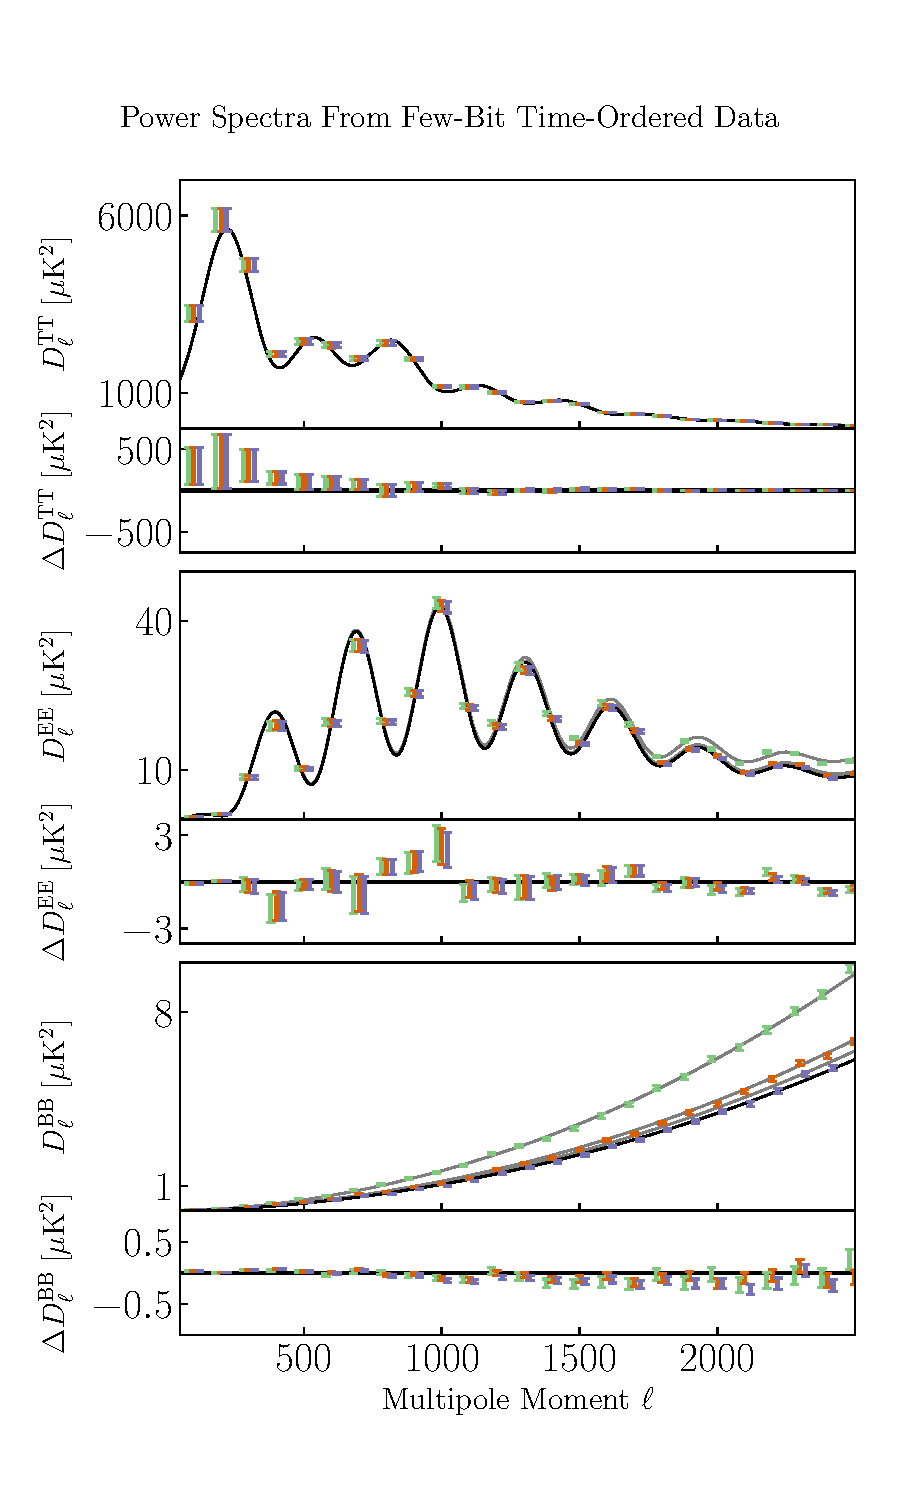
\includegraphics[width=0.5\textwidth,clip]{Plots/psrecovery.pdf}
  \caption[Current ]{
  Input power spectra used to generate the CMB template maps plus detector noise level (black) and power spectra using 3 bit TOD (violet). Simulations with $1,024,000$ hits per map pixel were used in this plot. No appreciable differences are visible for other depths of observation.
\label{fig:psrecover}
}
\end{figure}

\subsection{White Noise}
\label{subsec:whitenoise}

To investigate whether the noise added through digitisation has any $\ell$ dependence we subtract the template maps from the simulated observations. Beyond a calibration error, the power spectra of difference maps do not show any $\ell$ dependence in the added noise as seen in figure \ref{fig:diffpswn}. The plot also reveals that three bit digitisation performs best, followed by two bit and one bit. This is expected, because with each additional bit more information is retained.

% This is in agreement with (planck website) but does not match the results of (planck short paper). This is likely due to the intricities of the planck compression scheme differing to what is considered here. A full comparison is difficult in the absense of a detailed description of the simulations carried out in either paper.

\begin{figure}[htb]\centering
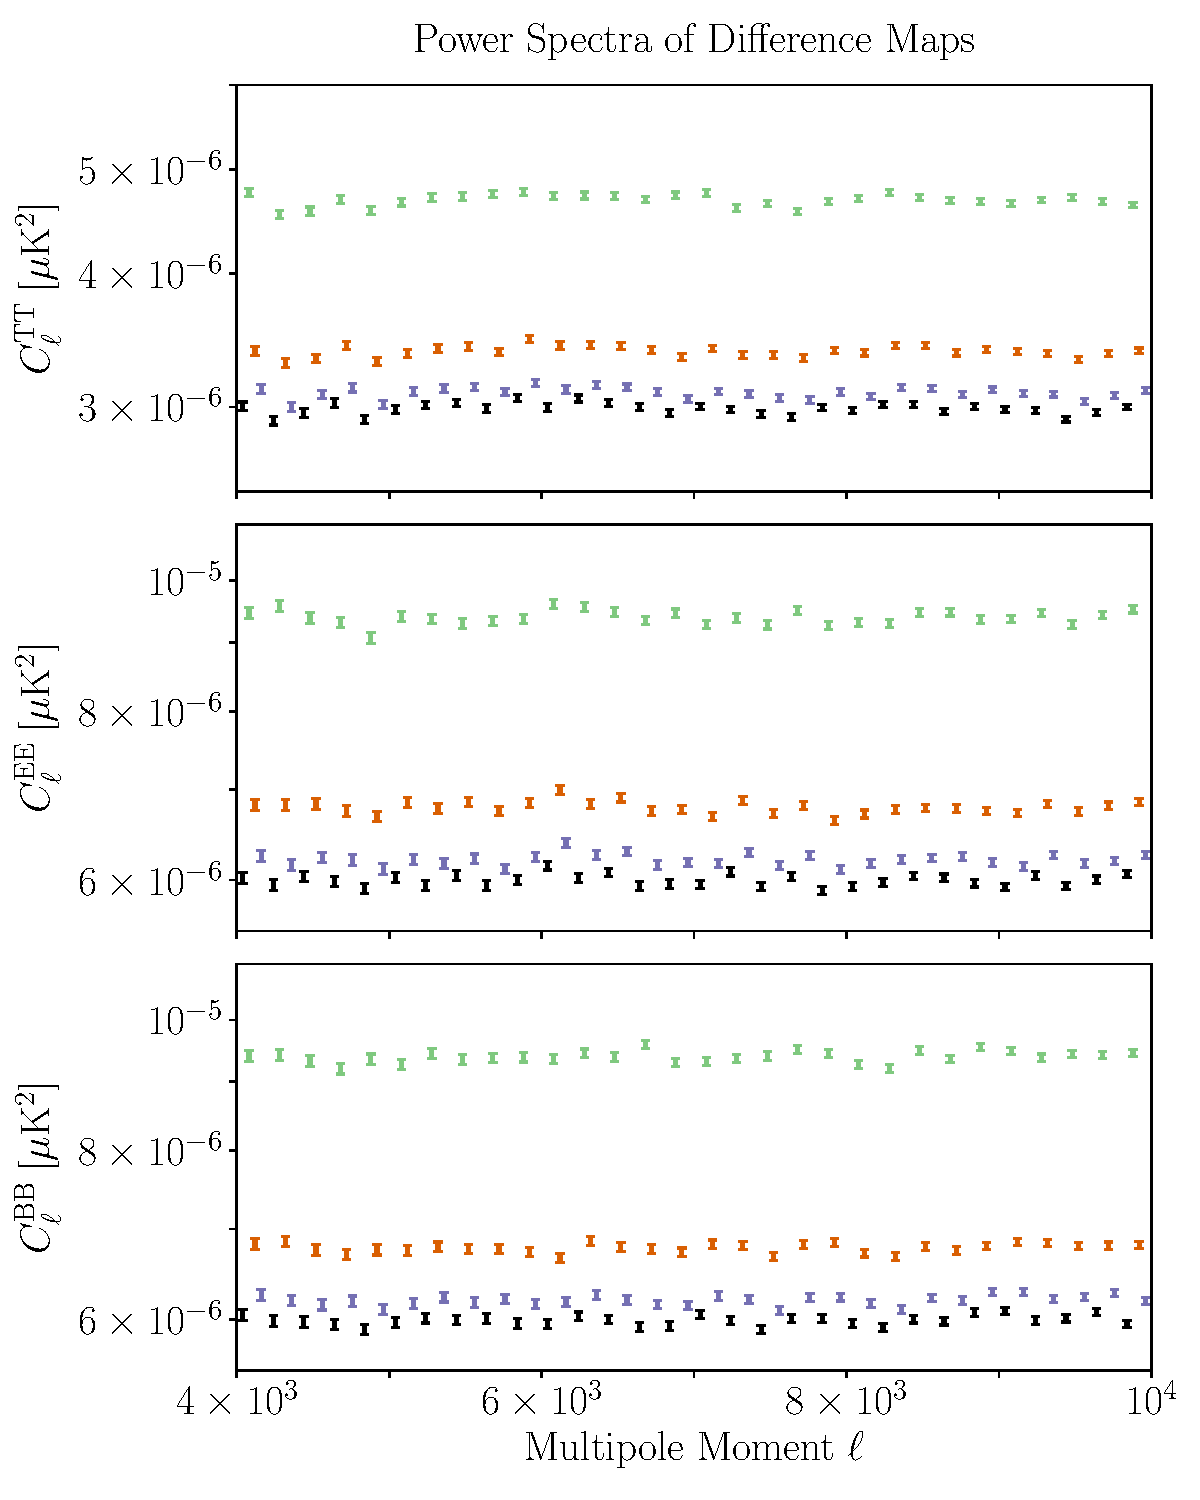
\includegraphics[width=0.5\textwidth,clip]{Plots/diffwn.pdf}
  \caption[Current ]{
  Power spectra of reconstructed minus input maps for one-bit (green), two-bit (orange), three-bit (violet) and the control case (black). No $\ell$ dependence is observed for all depths of observation. Simulations with $1,024,000$ hits per map pixel are shown.
\label{fig:diffpswn}
}
\end{figure}

To quantify the distortion caused by extreme digitisation we infer the map noise level from the relevant power spectra and compare them to the map noise level of control observations. We formulate

\begin{equation} \label{eq:extramapnoise}
\frac{\Delta \sigma}{\sigma} = \frac{\sigma_{\mathrm{map}}^{\mathrm{D}}-\sigma_{\mathrm{map}}^{\mathrm{C}}}{\sigma_{\mathrm{map}}^{\mathrm{C}}},
\end{equation}

where $\sigma_{\mathrm{map}}^{\mathrm{C}}$ and $\sigma_{\mathrm{map}}^{\mathrm{D}}$ are the map noise levels of control observations and simulations using few bit TOD respectively. Because we have seen no $\ell$ dependence in the power spectra of difference maps we presume digitisation to add a constant noise term. In the regime

\begin{equation} \frac{C_\ell^{\mathrm{N}}}{C_\ell^{\mathrm{S}}} \geq 10, \end{equation}

where $C_l^\mathrm{S}$ is the input CMB signal and $C_l^\mathrm{N}$ the detector noise level, power spectra are assumed to be noise dominated. Under this condition

\begin{equation} C_{\ell}^\mathrm{D} = C_\ell^\mathrm{N} + C_\ell^\mathrm{X}, \end{equation}

where $C_\ell^\mathrm{D}$ is the total power spectrum originating from a digitised timestream and $C_l^\mathrm{X}$ the additional noise induced through digitisation. We progress equation \ref{eq:extramapnoise} to

\begin{equation}\frac{\Delta \sigma}{\sigma} = \sqrt{\frac{C_l^\mathrm{D}}{C_l^{\mathrm{N}}}} - 1 = \sqrt{1 + \frac{C_\ell^\mathrm{X}}{C_\ell^{\mathrm{N}}}} - 1. \end{equation}

Before analysing $C_\ell^\mathrm{X}/C_\ell^\mathrm{N}$ we rebin the power spectra to $\Delta \ell \approx 100$. This ensures that points in the noise tail are independent, allowing us to extract an uncertainty for the above quantity.

The deduced additional noise for one, two, and three bit digitisation schemes is shown in table \ref{tab:extranoisewhite} in the appendix. We observe that $\Delta \sigma / \sigma$ is independent of the hits per pixel in the maps. This suggests that the additional noise scales in the same way as detector noise does. Furthermore, the compression performs equally well for temperature as it does for polarisation observations. Lastly, the added noise levels are low. When averaged over depth of observation and channel one bit digitisation adds $(24.8\pm 1.1)\%$ to the map noise level, two bit $(6.3\pm0.5)\%$ and three bit $(1.7\pm0.2)\%$. This is impressive, given that all schemes considered reduce TOD volume by at least an order of magnitude.

%communicate any information where in the first and last digitisation range ( $\left(x_N, \infty \right)$ and $\left( -\infty, x_1 \right)$ )the input signal lies.

%Extreme digitisation is a viable lossy compression technique when dealing with large volume, low signal to noise, slowly varying datasets. Making these assumptions the signal is small and constant for a considerable number of datapoints. For such an interval many samplings of the signal plus noise result in producing appropriate numbers in each output bin. The addition of more bits helps by classifying the size of the noise more accurately and hence approaching an improved estimate for the value of the signal faster. It is necessary to remain in the low signal to noise regime, as otherwise a dominant signal would saturate the digitisation scheme and for a given scheme only values in the range $\pm |N_{\mathrm{hits}}y_N|$ can be represented, given that we have $N_{\mathrm{hits}}$ datapoints. We must demand the data to be slowly varying such that many datapoints can be used to reconstruct a single significant step of the input signal. Finally a large data volume is clearly favourable for the reasons illustrated above: it allows for repeated sampling and therefore more accurate reconstruction of the weak signal.

\subsection{1/f Noise}
\label{subsec:oofnoise}

We follow up on the compelling results of the white noise case by implementing a more realistic noise profile. Ground-based CMB observations have $1/f$ noise spectra due to atmospheric effects \citep{lay2000}. We use the Fourier space noise profile

\begin{equation} \label{eq:1/fnoiseform}
\begin{aligned}
\left| N_{1/f}(\ell) \right|^2 &= \left| N\left(0, \sigma \right) \right|^2\\
&\times \left[ 1 + \left( \frac{\ell}{\lknee} \right)^{-3/2} \right]^2  exp\left[ -\left( \frac{\lcut}{\ell} \right)^{12} \right],
\end{aligned}
\end{equation}

where $N\left(0, \sigma \right)$ denotes a normally distributed random variable with mean $0$ and standard deviation $\sigma$. The first term on the second line produces $1/f$ behaviour and the second term on the same line suppresses the lowest modes. For temperature observations we choose $\lknee = 1000$ and $\lcut = 336$, to ensure that $|N_{1/f}(0.3\lknee)|^2 = |0.95 \sigma|^2$. For polarisation we set $\lknee = 50$ and $\lcut = 17$ for the same reason.

We use the same digitisation schemes as for white noise, but modify the parameter $\sigma$ in equations \ref{eq:1bit}, \ref{eq:2bit} and \ref{eq:3bit} by considering Parseval's theorem on the above noise profile. The appropriate value is obtained by evaluating the integral

\begin{equation}
\sigma^2 = \int_0^\infty \left| N_{1/f}(\ell) \right|^2 d\ell.
\end{equation}

We carry out the same simulations as described in subsection \ref{subsec:method} using the above noise profile and digitisation schemes for maps with $8,000$, $102,400$ and $1,024,000$ hits per pixel. HEALPix is used to calculate the spherical harmonics coefficients $a\ell m$. We mask the lowest modes in scan direction and obtain the power spectra. The analysis procedure of section \ref{subsec:whitenoise} is used to characterise the additional noise.

We recover similar results to the white noise case. As before three-bit performs the best, followed by two-bit and one-bit. The excess noise due to digitisation does not show any $\ell$ dependence and does not vary with the number of hits per pixel in the map. Temperature and polarisation observations incur the same noise penalty. Table \ref{tab:extranoiseoof} in the appendix displays the values of $\Delta \sigma / \sigma$ calculated. Averaging over depth of observation and channel we calculate that one bit digitisation adds $(27.7\pm 1.5)\%$ to the map noise level, two bit $(6.2\pm0.5)\%$ and three bit $(1.7\pm0.2)\%$. No significant deviations between white and $1/f$ noise results are found.

Extreme digitisation is a viable lossy compression technique when dealing with low signal to noise, large data sets, that have a slowly varying signal with respect to the sampling rate. These conditions allow us to reconstruct the underlying signal well. A small signal will also prevent saturation of the output, i.e. the inability of the digitised output to represent numbers larger than $y_N N_{\mathrm{hit}}$ or smaller than $y_1 N_{\mathrm{hit}}$, where $N_{\mathrm{hit}}$ is the number of data points in an interval. These conditions are satisfied by CMB data and our findings reflect this.

\section{Conclusion}
\label{sec:conclusions}

In this work we have motivated the investigation of extreme digitisation as a technique in combating potential challenges of CMB experiments. The reduction of TOD by an order of magnitude addresses potential issues in transmission from remote locations. Benefits in mission planning, data analysis and hardware requirements are possible.

We derived a set of one, two, and three bit digitisation schemes assuming white detector noise. Through simulated observation we determined the distortion this compression technique causes in temperate and polarisation power spectra. We find that an optimal three bit digitisation adds as little as $1.7\%$ to the map noise level for temperature and polarisation observations alike. No change in the results is observed for maps of different hits per pixel and no $\ell$ dependence was observed in the added noise. Extending the model to more realistic $1/f$ detector noise did not change these results.

The additional noise is insignificant for ground-based experiments, which increase their detector count by orders of magnitude between generations. Space-based experiments which have their own unique issues may consider this noise penalty problematic.

Future work investigating this compression technique must aim to understand the nature of the induced noise better. It is of great value to find the higher statistical moments, i.e. skewness and kurtosis, of the added noise term. For this an analysis of the performance of cluster-finding algorithms on the digitised TOD is recommended.

\acknowledgments % thank patrick for discussion/starting point? Andrew?

% Melbourne CMB group, funding, NERSC.

We thank the \changed{referee as well as} Srinivasan Raghunathan and Federico Bianchini for valuable feedback on the manuscript. 
We acknowledge support from an Australian Research Council Future Fellowship (FT150100074), and also from the University of Melbourne. 
This research used resources of the National Energy Research Scientific Computing Center, which is supported by the Office of Science of the U.S. Department of Energy under Contract No. DE-AC02-05CH11231. 
We acknowledge the use of the Legacy Archive for Microwave Background Data Analysis (LAMBDA). Support for LAMBDA is provided by the NASA Office of Space Science.

% all code stuff

This research made use of the NumPy \citep{numpy}, SciPy \citep{scipy}, Matplotlib \citep{matplotlib}, and Astropy \citep{astropy} packages.

\newpage

% APPENDIX
\appendix

% result tables
\subsection{Digitisation Noise Levels}
\label{subsec:appendixnoisetables}

\def\arraystretch{1.3}
\begin{table*}[tbh]
\begin{center}
\caption{\label{tab:extranoisewhite} Additional Noise - White Detector Noise}
\small
\begin{tabular}{c c c c c}
Hits Per Pixel & Channel & 1 Bit & 2 Bit & 3 Bit \\
\hline
\hline
\multirow{3}{*}{$800$}  & TT  & $ 0.252 \pm 0.009 $  & $ 0.064 \pm 0.003 $  & $ 0.017 \pm 0.002 $ \\
& EE  & $ 0.253 \pm 0.012 $  & $ 0.064 \pm 0.005 $  & $ 0.017 \pm 0.004 $ \\
& BB  & $ 0.254 \pm 0.011 $  & $ 0.065 \pm 0.005 $  & $ 0.018 \pm 0.004 $ \\
\hline
\multirow{3}{*}{$8,000$}  & TT  & $ 0.252 \pm 0.008 $  & $ 0.064 \pm 0.003 $  & $ 0.017 \pm 0.002 $ \\
& EE  & $ 0.252 \pm 0.007 $  & $ 0.064 \pm 0.004 $  & $ 0.017 \pm 0.002 $ \\
& BB  & $ 0.252 \pm 0.018 $  & $ 0.063 \pm 0.009 $  & $ 0.018 \pm 0.004 $ \\
\hline
\multirow{3}{*}{$80,000$}  & TT  & $ 0.249 \pm 0.011 $  & $ 0.064 \pm 0.005 $  & $ 0.018 \pm 0.002 $ \\
& EE  & $ 0.250 \pm 0.011 $  & $ 0.064 \pm 0.005 $  & $ 0.018 \pm 0.002 $ \\
& BB  & $ 0.248 \pm 0.018 $  & $ 0.063 \pm 0.009 $  & $ 0.018 \pm 0.003 $ \\
\hline
\multirow{3}{*}{$1,024,000$}  & TT  & $ 0.25 \pm 0.009 $  & $ 0.063 \pm 0.003 $  & $ 0.017 \pm 0.002 $ \\
& EE  & $ 0.252 \pm 0.008 $  & $ 0.065 \pm 0.003 $  & $ 0.018 \pm 0.002 $ \\
& BB  & $ 0.252 \pm 0.008 $  & $ 0.064 \pm 0.004 $  & $ 0.017 \pm 0.002 $ \\
\hline
\multirow{3}{*}{$10,240,000$}  & TT  & $ 0.186 \pm 0.025 $  & $ 0.046 \pm 0.007 $  & $ 0.013 \pm 0.002 $ \\
& EE  & $ 0.253 \pm 0.009 $  & $ 0.065 \pm 0.004 $  & $ 0.018 \pm 0.002 $ \\
& BB  & $ 0.252 \pm 0.012 $  & $ 0.064 \pm 0.004 $  & $ 0.018 \pm 0.002 $ \\
\hline
\multirow{3}{*}{$102,400,000$}  & TT  & $ 0.246 \pm 0.005 $  & $ 0.063 \pm 0.002 $  & $ 0.017 \pm 0.001 $ \\
& EE  & $ 0.251 \pm 0.008 $  & $ 0.064 \pm 0.004 $  & $ 0.018 \pm 0.002 $ \\
& BB  & $ 0.252 \pm 0.009 $  & $ 0.064 \pm 0.003 $  & $ 0.018 \pm 0.002 $ \\
\hline
\multicolumn{2}{c}{Average}  & $ 0.248 \pm 0.011 $  & $ 0.063 \pm 0.005 $  & $ 0.017 \pm 0.002 $ \\
\end{tabular}
\tablecomments{ 
Percent addition to the map noise level $\Delta \sigma / \sigma$ due to one, two, and three bit digitisation for white detector noise. We notice that there is no appreciable variation with depth of observations and channel for a given digitisation scheme.
} \normalsize
\end{center}
\end{table*}

\def\arraystretch{1.3}
\begin{table*}[tbh]
\begin{center}
\caption{\label{tab:extranoiseoof} Additional Noise - $1/f$ Detector Noise}
\small
\begin{tabular}{c c c c c}
Hits Per Pixel & Channel & 1 Bit & 2 Bit & 3 Bit \\
\hline
\hline
\multirow{3}{*}{$8,000$}  & TT  & $ 0.231 \pm 0.017 $  & $ 0.058 \pm 0.005 $  & $ 0.016 \pm 0.002 $ \\
& EE  & $ 0.300 \pm 0.012 $  & $ 0.064 \pm 0.004 $  & $ 0.018 \pm 0.002 $ \\
& BB  & $ 0.294 \pm 0.022 $  & $ 0.062 \pm 0.007 $  & $ 0.017 \pm 0.003 $ \\
\hline
\multirow{3}{*}{$102,400$}  & TT  & $ 0.235 \pm 0.014 $  & $ 0.06 \pm 0.004 $  & $ 0.017 \pm 0.002 $ \\
& EE  & $ 0.299 \pm 0.009 $  & $ 0.064 \pm 0.004 $  & $ 0.017 \pm 0.002 $ \\
& BB  & $ 0.298 \pm 0.025 $  & $ 0.064 \pm 0.007 $  & $ 0.018 \pm 0.002 $ \\
\hline
\multirow{3}{*}{$1,024,000$}  & TT  & $ 0.238 \pm 0.013 $  & $ 0.06 \pm 0.005 $  & $ 0.017 \pm 0.002 $ \\
& EE  & $ 0.299 \pm 0.008 $  & $ 0.063 \pm 0.004 $  & $ 0.017 \pm 0.002 $ \\
& BB  & $ 0.299 \pm 0.010 $  & $ 0.064 \pm 0.005 $  & $ 0.018 \pm 0.002 $ \\
\hline
\multicolumn{2}{c}{Average}  & $ 0.277 \pm 0.015 $  & $ 0.062 \pm 0.005 $  & $ 0.017 \pm 0.002 $ \\
\end{tabular}
\tablecomments{ 
Percent addition to the map noise level $\Delta \sigma / \sigma$ due to one, two, and three bit digitisation for $1/f$ detector noise. As in the white noise case we observe no significant trend with the numbers of hits per map pixel or channel for a given digitisation scheme. No significant deviation in the values compared to simulations assuming white detector noise exists.
} \normalsize
\end{center}
\end{table*}


% Power preservation theoretical calculation
\subsection{Preserving Power in Digitised Data}
\label{subsec:appendixpreservepower}

As mentioned in subsection \ref{subsec:extremedigitisation} the designed digitisation schemes do not conserve power. This is because the distortion metric used does not demand this. We can ensure power preservation by multiplying the output by a constant $\mathcal{N}$. In the following we will show that this is true and derive an expression for $\mathcal{N}$.

We demand equal cross power in input and output, i.e.

\begin{equation} \label{eq:normcrosspower}
\langle s_1 s_2 \rangle = \mathcal{N} \langle D(s_1) D(s_2) \rangle,
\end{equation}

where timestreams $s_{1,2}$ sample the same underlying signal, $\mu$, but add different noise realisations $\xi_{1, 2}$. The digitisation process is denoted by $D(\dots)$. We begin by looking at the crosspower of non-digitised timestreams

\begin{equation}
\langle s_1 s_2 \rangle = \langle (\mu + \xi_1) (\mu + \xi_2) \rangle =  \langle \mu^2 \rangle = \mu^2.
\end{equation}

This allows us to state

\begin{equation}
cov(s_1, s_2) = \langle s_1 s_2 \rangle - \langle s_1 \rangle \langle s_2 \rangle = \mu^2 - \mu^2 = 0.
\end{equation}

We argue that this still holds true after the digitisation process, since timestreams still have independent stochastic components. Digitisation discretises the probability distributions at play, but does not change the underlying dynamics.

\begin{equation}
\langle D(s_1) D(s_2) \rangle = \sum_1 \sum_2 D(\mu + \xi_1) D(\mu + \xi_1) P(D(\mu + \xi_1)) P(D(\mu + \xi_2)),
\end{equation}

where $P$ denotes the probability of a certain digitisation level occurring. We now assume that the underlying signal is small, i.e. $| \mu | \ll | \xi |$. This is true for ground-based CMB observations. In this limit $D(\mu + \xi)$ is digitised to the same value as $D(\xi)$. The probabilities can then be expressed as integrals over the relevant sections of correctly parameterised probability distributions. We proceed by assuming that noise is drawn from normal distributions with mean $\mu$ and standard deviation $\sigma$, i.e. $N(\mu, \sigma, \xi)$.

\begin{equation}
\langle D(s_1) D(s_2) \rangle = \sum_{i=0}^N \sum_{j=0}^N  \int_{x_i}^{x_{i+1}} \int_{x_j}^{x_{j+1}} y_i y_j N(\mu, \sigma, \xi_1) N(\mu, \sigma, \xi_2) d\xi_1 d\xi_2.
\end{equation}

We separate the above sums temporarily to detail our next steps. We split up the integrals over ranges that allow us to recognise the error function evaluated at different points.

\begin{equation}
\langle D(s_1) D(s_2) \rangle = \left[ \sum_{i=0}^N  y_i \int_{x_i}^{x_{i+1}} N(\mu, \sigma)  d\xi_1 \right] \left[  \sum_{j=0}^N y_j \int_{x_j}^{x_{j+1}} N(\mu, \sigma)d\xi_2 \right].
\end{equation}

\begin{equation}
= \left\{ \sum_{i=0}^N  y_i \left[ \int_{-\infty}^{x_{i+1}} - \int_{-\infty}^{x_{i}} \right] N(\mu, \sigma)  d\xi_1 \right\} \left\{  \sum_{j=0}^N y_j \left[ \int_{-\infty}^{x_{j+1}} - \int_{-\infty}^{x_{j}} \right] N(\mu, \sigma)d\xi_2 \right\}.
\end{equation}

\begin{equation}
= \left\{ \sum_{i=0}^N  \frac{y_i}{2} \left[ erf \left( \frac{x_{i+1} - \mu}{\sqrt{2}\sigma} \right) - erf \left( \frac{x_{i} - \mu}{\sqrt{2}\sigma} \right) \right] \right\} \left\{  \sum_{j=0}^N \frac{y_j}{2} \left[ erf \left( \frac{x_{j+1} - \mu}{\sqrt{2}\sigma} \right) - erf \left( \frac{x_{j} - \mu}{\sqrt{2}\sigma} \right) \right] \right\}.
\end{equation}

Using the Maclaurin series of the error function

\begin{equation}
\begin{aligned}
\langle D(s_1) D(s_2) \rangle &= \left\{ \sum_{i=0}^N  \frac{y_i}{2} \left[ \frac{2}{\sqrt{\pi}} \sum_{n = 0}^\infty \frac{(-1)^n}{n! (2n+1)} \frac{1}{(\sqrt{2}\sigma)^{2n+1}} \left( (x_{i+1}-\mu)^{2n+1} - (x_{i}-\mu)^{2n+1} \right) \right] \right\} \\
&\times \left\{ \sum_{j=0}^N  \frac{y_j}{2} \left[ \frac{2}{\sqrt{\pi}} \sum_{m = 0}^\infty \frac{(-1)^m}{m! (2m+1)} \frac{1}{(\sqrt{2}\sigma)^{2m+1}} \left( (x_{j+1}-\mu)^{2m+1} - (x_{j}-\mu)^{2m+1} \right) \right] \right\}
\end{aligned}.
\end{equation}

The binomial expansion is now applied to all brackets containing $\mu$ and the sums over $n$ and $m$ are recombined

\begin{equation}
\begin{aligned}
\langle D(s_1) D(s_2) \rangle &= \left\{ \sum_{i=0}^N  \frac{y_i}{\sqrt{pi}} \left[ \sum_{n = 0}^\infty \frac{(-1)^n}{n! (2n+1)} \frac{1}{(\sqrt{2}\sigma)^{2n+1}} \left( \sum_{k=0}^{2n+1} {2n+1 \choose k} \mu^k ( x_{i+1}^{2n+1-k} - x_{i}^{2n+1-k} ) \right) \right] \right\} \\
&\times \left\{ \sum_{j=0}^N  \frac{y_j}{\sqrt{2}} \left[ \sum_{m = 0}^\infty \frac{(-1)^m}{m! (2m+1)} \frac{1}{(\sqrt{2}\sigma)^{2m+1}} \left( \sum_{l=0}^{2m+1} {2m+1 \choose l} \mu^l ( x_{j+1}^{2m+1-l} - x_{j}^{2m+1-l} ) \right) \right] \right\}.
\end{aligned}
\end{equation}

\begin{equation}
\begin{aligned}
&= \sum_{i,j=0}^N  \frac{y_i y_j}{\pi} \left[ \sum_{n,m = 0}^\infty \frac{1}{n! (2n+1)} \frac{(-1)^{n+m}}{m! (2m+1)} \frac{1}{(\sqrt{2}\sigma)^{2n+2m+2}} \right. \\
& \left. \times \left( \sum_{k, l = 0}^{2n+1} {2n+1 \choose k} {2m+1 \choose l} \mu^{k+l} ( x_{i+1}^{2n+1-k} - x_{i}^{2n+1-k} ) ( x_{j+1}^{2m+1-l}- x_{j}^{2m+1-l}) \right) \right].
\end{aligned}
\end{equation}

\begin{equation} \label{eq:dcompleteklsum}
=  \frac{1}{\pi} \sum_{n,m = 0}^\infty \frac{1}{n! (2n+1)} \frac{(-1)^{n+m}}{m! (2m+1)} \frac{1}{(\sqrt{2}\sigma)^{2n+2m+2}} \sum_{k, l = 0}^{2n+1} {2n+1 \choose k} {2m+1 \choose l} \mu^{k+l} \sum_{i,j=0}^N y_i y_j \psi^{k, n}_i \psi^{l, m}_j,
\end{equation}

where in the last line we have moved $y_i$ and $y_j$ and the sum over $i,j$ as far forward as possible. Additionally, we have introduced the new variable

\begin{equation}
\psi_i^{k,n} = x_{i+1}^{2n+1-k} - x_{i}^{2n+1-k}.
\end{equation}

We now split the innermost term such that

\begin{equation}
\sum_{i,j = 0}^N y_i y_j \psi_i^{k, n} \psi_j^{l, m} = \left( \sum_{i = 0}^{N/2}\sum_{j = 0}^{N/2} + \sum_{i = N/2}^{N}\sum_{j = 0}^{N/2} + \sum_{i = 0}^{N/2}\sum_{j = N/2}^{N} + \sum_{i = N/2}^{N}\sum_{j = N/2}^{N} \right) y_i y_j \psi_i^{k, n} \psi_j^{l, m}.
\end{equation}

\begin{equation}
 = \sum_{i = 0}^{N/2}\sum_{j = 0}^{N/2} y_i y_j \psi_i^{k, n} \psi_j^{l, m} + \sum_{i = 0}^{N/2}\sum_{j = 0}^{N/2} y_{N-i} y_j \psi_{N-i}^{k, n} \psi_j^{l, m} + \sum_{i = 0}^{N/2}\sum_{j = 0}^{N/2} y_i y_{N-j} \psi_i^{k, n} \psi_{N-j}^{l, m} + \sum_{i = 0}^{N/2}\sum_{j = 0}^{N/2} y_{N-i} y_{N-j} \psi_{N-i}^{k, n} \psi_{N-j}^{l, m},
\end{equation}

where we have shifted all indices of sums that do not start at $0$ to $N-i$ and/or $N-j$ as applicable. We recombine the sums such that

\begin{equation}
\sum_{i,j = 0}^N y_i y_j \psi_i^{k, n} \psi_j^{l, m} = \sum_{i = 0}^{N/2}\sum_{j = 0}^{N/2} \left( y_i y_j \psi_i^{k, n} \psi_j^{l, m} +  y_{N-i} y_j \psi_{N-i}^{k, n} \psi_j^{l, m} + y_i y_{N-j} \psi_i^{k, n} \psi_{N-j}^{l, m} + y_{N-i} y_{N-j} \psi_{N-i}^{k, n} \psi_{N-j}^{l, m} \right)
\end{equation}

A digitisation scheme designed according to the distortion metric in section \ref{subsec:extremedigitisation} for normally distributed noise will satisfy $y_i = -y_{N-i}$ and $x_i = -x_{N+1-i}$.  This simply states symmetry of the digitisation thresholds and levels about zero or after a mean has been subtracted. With this information we can condense the above to

\begin{equation} \label{eq:ijsum}
\sum_{i,j = 0}^N y_i y_j \psi_i^{k, n} \psi_j^{l, m} = \sum_{i = 0}^{N/2}\sum_{j = 0}^{N/2} y_i y_j \left( \psi_i^{k, n} \psi_j^{l, m} - \psi_{N-i}^{k, n} \psi_j^{l, m} - \psi_i^{k, n} \psi_{N-j}^{l, m} + \psi_{N-i}^{k, n} \psi_{N-j}^{l, m} \right)
\end{equation}

We keep hold of this result and move onto the double sum over $k,l$ in equation \ref{eq:dcompleteklsum}. Since we assumed that the signal is small we would like to calculate the leading order contributions in $\mu$. We split up the double sum such that

\begin{equation} \label{eq:ksums}
\sum_{k, l = 0}^{2n+1} = \sum_{\mathrm{even} \> k}^{2n+1} \sum_{\mathrm{even} \> l}^{2n+1}  + \sum_{\mathrm{odd} \> k}^{2n+1} \sum_{\mathrm{odd} \> l}^{2n+1} + \sum_{\mathrm{odd} \> k}^{2n+1} \sum_{\mathrm{even} \> l}^{2n+1}  + \sum_{\mathrm{even} \> k}^{2n+1} \sum_{\mathrm{odd} \> l}^{2n+1}.
\end{equation}

The first two terms in the above will lead to even powers of $\mu$ whereas the last two will lead to odd powers of $\mu$. Before we can look at these terms in more detail we need to see how the index shift $i \to N-i$ affects $\psi_{i}^{k, n}$.

\begin{equation}
\begin{aligned}
\psi_{N-i}^{k,n} &= x_{N+1-i}^{2n+1-k} - x_{N-i}^{2n+1-k} = (-x_{i})^{2n+1-k} - (-x_{i+1})^{2n+1-k}\\
&= (-1)^{2n+1-k} (x_{i})^{2n+1-k} - x_{i+1})^{2n+1-k} ) = (-1)^{2n+2-k} (x_{i+1})^{2n+1-k} - x_{i1})^{2n+1-k} )\\
&= (-1)^{k} \psi_{i}^{k,n}.
\end{aligned}
\end{equation}

We are now ready to put all pieces together. We start by investigating even powers of $\mu$ in equation \ref{eq:dcompleteklsum} that arise from even $k$ and $l$. Under the assumptions made \ref{eq:ijsum} reduces to

\begin{equation}
\sum_{i,j = 0}^N y_i y_j \psi_i^{k, n} \psi_j^{l, m} = \sum_{i = 0}^{N/2}\sum_{j = 0}^{N/2} y_i y_j  \left( \psi_i^{k, n} \psi_j^{l, m} - \psi_{i}^{k, n} \psi_j^{l, m} - \psi_i^{k, n} \psi_{j}^{l, m} + \psi_{i}^{k, n} \psi_{j}^{l, m} \right) = 0.
\end{equation}

The term vanishes. The other way of producing even powers of $\mu$ in equation \ref{eq:dcompleteklsum} is with odd $k$ and $l$. These assumptions simplify equation \ref{eq:ijsum} to

\begin{equation}
\sum_{i,j = 0}^N y_i y_j \psi_i^{k, n} \psi_j^{l, m} = \sum_{i = 0}^{N/2}\sum_{j = 0}^{N/2} y_i y_j \left( \psi_i^{k, n} \psi_j^{l, m} + \psi_{i}^{k, n} \psi_j^{l, m} + \psi_i^{k, n} \psi_{j}^{l, m} + \psi_{i}^{k, n} \psi_{j}^{l, m} \right) = 4 \sum_{i = 0}^{N/2}\sum_{j = 0}^{N/2} y_i y_j \psi_i^{k, n} \psi_j^{l, m}.
\end{equation}

This term survives and leads to even powers of $\mu$ in equation \ref{eq:dcompleteklsum}. Moving on to odd powers of $\mu$ we consider the case of odd $k$ and even $l$. We observe

\begin{equation}
\sum_{i,j = 0}^N y_i y_j \psi_i^{k, n} \psi_j^{l, m} = \sum_{i = 0}^{N/2}\sum_{j = 0}^{N/2} y_i y_j \left( \psi_i^{k, n} \psi_j^{l, m} + \psi_{i}^{k, n} \psi_j^{l, m} - \psi_i^{k, n} \psi_{j}^{l, m} - \psi_{i}^{k, n} \psi_{j}^{l, m} \right) = 0
\end{equation}

and similarly

\begin{equation}
\sum_{i,j = 0}^N y_i y_j \psi_i^{k, n} \psi_j^{l, m} = \sum_{i = 0}^{N/2}\sum_{j = 0}^{N/2} y_i y_j \left( \psi_i^{k, n} \psi_j^{l, m} - \psi_{i}^{k, n} \psi_j^{l, m} + \psi_i^{k, n} \psi_{j}^{l, m} - \psi_{i}^{k, n} \psi_{j}^{l, m} \right) = 0\\
\end{equation}

for odd $k$ and even $l$. All odd powers of $\mu$ in equation \ref{eq:dcompleteklsum} vanish. Moreover we can also state that there is no $\mu$ independent term, since this could only be produced by $k=l=0$, but even $k$ and $l$ terms are shown to vanish. Therefore

\begin{equation}
\langle D(s_1) D(s_2) \rangle = c \mu^2 + \mathcal{O}(\mu^4)
\end{equation}

where $c$ is some constants that depend on the specific digitisation scheme chosen. We now have prove that in the small signal limit and under the assumptions about the digitisation scheme stated normalisation can indeed be achieved by a constant. Returning to equation \ref{eq:normcrosspower} we see

\begin{equation}
\mathcal{N}  = \frac{\langle s_1 s_2 \rangle}{\langle D(s_1) D(s_2) \rangle} = \frac{\mu^2}{c \mu^2 + \mathcal{O}(\mu^4)} = \frac{1}{c + \mathcal{O}(\mu^2)} = \frac{1}{c},
\end{equation}

where we have ignored higher order contributions. From equation \ref{eq:dcompleteklsum} we obtain an expression for $\mathcal{N}$. We focus on $k=l=1$ terms.

\begin{equation}
\begin{aligned}
c = \sum_{i,j=0}^N  \frac{y_i y_j}{\pi} \left[ \sum_{n,m = 0}^\infty \frac{1}{n! (2n+1)} \frac{(-1)^{n+m}}{m! (2m+1)} \frac{1}{(\sqrt{2}\sigma)^{2n+2m+2}} \left( {2n+1 \choose 1} {2m+1 \choose 1} ( x_{i+1}^{2n} - x_{i}^{2n} ) ( x_{j+1}^{2m} - x_{j}^{2m} ) \right) \right]
\end{aligned}
\end{equation}

\begin{equation}
c = \sum_{i,j=0}^N  \frac{y_i y_j}{\pi} \left[ \sum_{n,m = 0}^\infty \frac{1}{n! (2n+1)} \frac{(-1)^{n+m}}{m! (2m+1)} \frac{1}{(\sqrt{2}\sigma)^{2n+2m+2}} \left( \frac{(2n+1)!}{(2n)!} \frac{(2m+1)!}{(2m)!} ( x_{i+1}^{2n} - x_{i}^{2n} ) ( x_{j+1}^{2m} - x_{j}^{2m} ) \right) \right]
\end{equation}

\begin{equation}
c = \sum_{i,j=0}^N \frac{y_i y_j}{2\pi\sigma^2} \left[ \sum_{n = 0}^\infty \frac{(-1)^n}{n!} \frac{1}{(\sqrt{2}\sigma)^{2n}}  ( x_{i+1}^{2n} - x_{i}^{2n} ) \right] \left[ \sum_{m = 0}^\infty \frac{(-1)^m}{m!} \frac{1}{(\sqrt{2}\sigma)^{2m}} ( x_{j+1}^{2m} - x_{j}^{2m} ) \right].
\end{equation}

We recognise the exponential function in the above.

\begin{equation}
c = \sum_{i,j=0}^N \frac{y_i y_j}{2\pi\sigma^2} \left\{ exp \left[ - \left(\frac{x_{i+1}}{\sqrt{2}\sigma} \right)^2 \right] - exp \left[ - \left(\frac{x_{i}}{\sqrt{2}\sigma} \right)^2 \right] \right\} \left\{ exp \left[ - \left(\frac{x_{j+1}}{\sqrt{2}\sigma} \right)^2 \right] - exp \left[ - \left(\frac{x_{j}}{\sqrt{2}\sigma} \right)^2 \right] \right\}
\end{equation}

The normalisation constant therefore is given by

\begin{equation}
\mathcal{N} = \left( \sum_{i,j=0}^N \frac{y_i y_j}{2\pi\sigma^2} \left\{ exp \left[ - \left(\frac{x_{i+1}}{\sqrt{2}\sigma} \right)^2 \right] - exp \left[ - \left(\frac{x_{i}}{\sqrt{2}\sigma} \right)^2 \right] \right\} \left\{ exp \left[ - \left(\frac{x_{j+1}}{\sqrt{2}\sigma} \right)^2 \right] - exp \left[ - \left(\frac{x_{j}}{\sqrt{2}\sigma} \right)^2 \right] \right\} \right)^{-1}
\end{equation}

This can be calculated for a given digitisation scheme $N, x_i, y_i$ and standard deviation of noise $\sigma$. Notice that if the digitisation scheme is chosen such that $y_i$ and $x_i$ depend linearly on $\sigma$ the normalisation constant is independent of $\sigma$.

\newpage

\bibliography{digitisation}


\end{document}
